\chapter{Online Connection CD}

\begin{figure}[H]
    \centering
    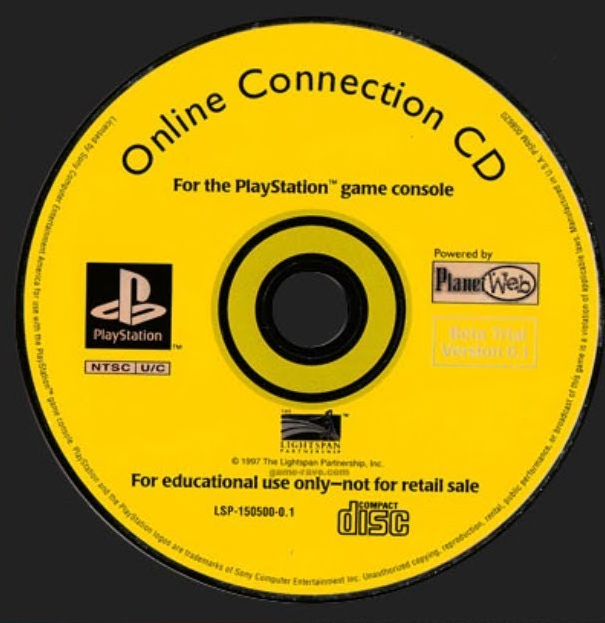
\includegraphics[width=0.5\textwidth]{./Games/OnlineConnectionCD/Images/OnlineConnectionCDDisk.png}
    \caption{Online Connection CD Disk}
\end{figure}

\section{Overview}

The Online Connection CD is perhaps one of the strangest, but at the same time most interesting pieces of media around.
There is very little information surrounding this particular piece of media, but the vast majority of the information that I discover about this CD comes from this video by GameRaveTV: \url{https://www.youtube.com/watch?v=kv3_cspRndY}.
This video is perhaps the best resource for information pertaining to the Online Connection CD, and specifically the incredible variety of issues that GameRaveTV had to go through in order to get even a degree of functionality.
It has much more specific information about the Online Connection CD than what is presented here, and I would highly recommend watching it if you are interested in more specific information than what will be discussed here.

In spite of this video however, I would still like to add a bit of context to the situation with the state of online functionality on the PlayStation 1 at the time.

The Lightspan Partnership actually reached out to an estimated 3,600 schools within the United States to get a lot of their software into schools.
Out of these 3,600, there were also a very small number of schools which received the Online Connection CD, almost as a testing ground for the software.
The Online Connection CD was a CD that was sent out to schools to help teachers and students gain access to the internet.
This was in opposition to desktop computers of course, which, at the time, were much more expensive than a PlayStation console.

When you placed the Online Connection CD into the PlayStation, with an accompanying modem and memory card, you were presented with a web browser that allows you to access the internet, and send emails.
However, given that the CD was released in 1997, the disk no longer works in opening a web browser, or loading any web pages.

This is not just perhaps one of the strangest products that Lightspan ever released, but also perhaps one of the strangest products that was ever released for the PlayStation 1.
As far as I am aware, the only other way to access the internet on the PlayStation 1 was using a GameShark.

Another resource of information for the Online Connection CD is this guide on GameFAQs: \url{https://gamefaqs.gamespot.com/ps/205836-lightspan-online-connection-cd/faqs/75191}.
This guide is a bit more technical than the GameRaveTV video, and goes into a bit more detail about the technical aspects of the Online Connection CD.

Another website for technical detail is this web page capture by the wayback machine: \url{https://web.archive.org/web/20170822221459/https://game-rave.com/?gamepress_reviews=lightspan-online-connection-cd#}.

\begin{figure}[H]
    \centering
    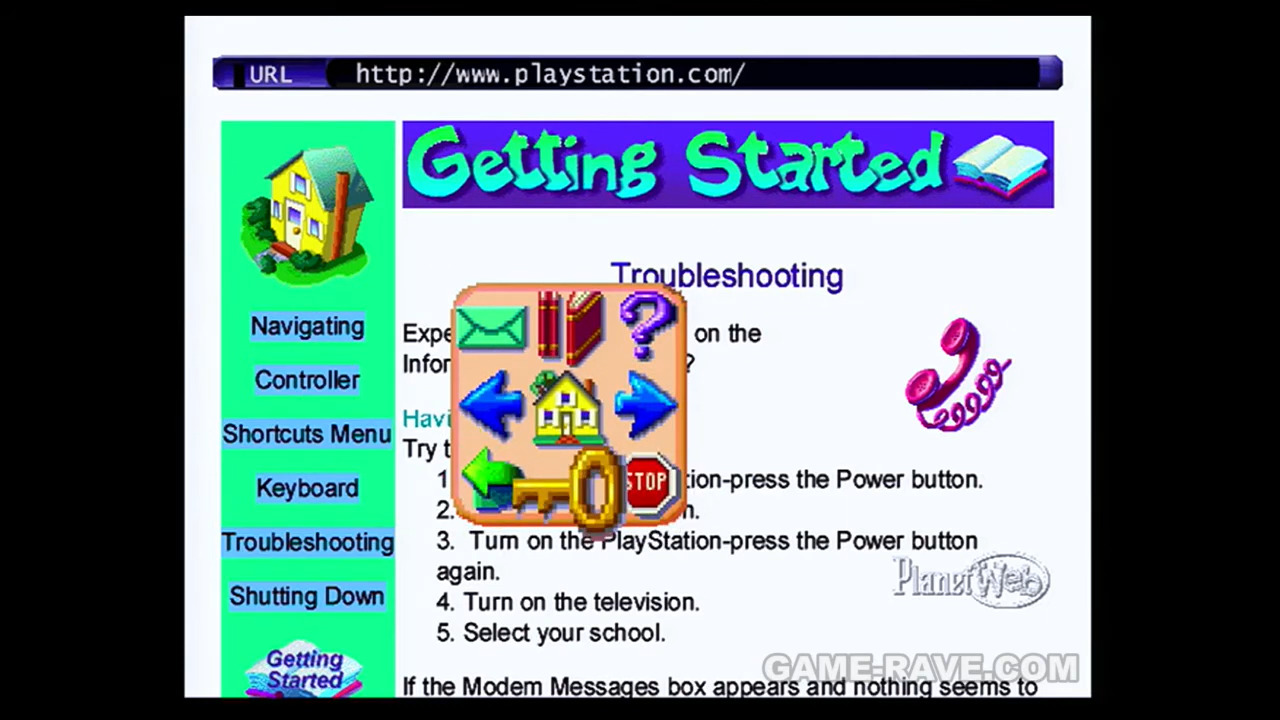
\includegraphics[width=0.5\textwidth]{./Games/OnlineConnectionCD/Images/OnlineConnectionsCDExampleWebpage.jpg}
    \caption{Online Connection CD Example Webpage}
\end{figure}

\begin{figure}[H]
    \centering
    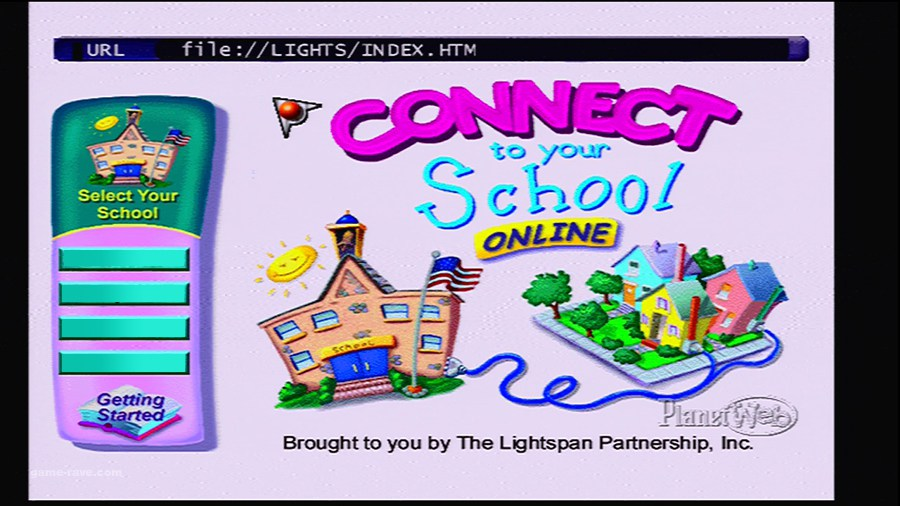
\includegraphics[width=0.5\textwidth]{./Games/OnlineConnectionCD/Images/OnlineConnectionsCDStartScreen.jpg}
    \caption{Online Connection CD Start Screen}
\end{figure}